%% Original Software Publication article for Elsevier's `elsarticle' class
%% Target journal: Neurocomputing

\documentclass[preprint,12pt,a4paper]{elsarticle}

% -------------------------
% Packages
% -------------------------
\usepackage[a4paper,margin=2.5cm]{geometry}
\usepackage{amssymb}
\usepackage{amsmath}
\usepackage{graphicx}
\graphicspath{{figures/}}
\usepackage{subcaption}
\usepackage{placeins}
\usepackage[font=small,labelfont=bf]{caption}
\usepackage{tabularray}
\usepackage{booktabs,tabularx,makecell,threeparttable,adjustbox}
\usepackage{array}
\usepackage[table]{xcolor}
\definecolor{rowgray}{gray}{0.96}
\newcommand{\best}[1]{\textbf{#1}}
\newcommand{\second}[1]{\underline{#1}}
\usepackage{xurl}
\usepackage[hidelinks]{hyperref}
\usepackage{tikz}
\usetikzlibrary{arrows.meta,positioning,backgrounds}

\newcommand{\theratimeRepository}{\url{https://github.com/briouyaasmae/theratime}}
\newcommand{\theratimeZenodo}{10.5281/zenodo.20058732}

\journal{Neurocomputing}

\begin{document}

\begin{frontmatter}

\title{TheraTime: a reliability-aware software framework for therapeutic timing evaluation in mental-health response retrieval}

\author[label1]{Asmae Briouya\corref{cor1}}
\cortext[cor1]{Corresponding author.}
\ead{asmae.briouya@uit.ac.ma}
\author[label1]{Hasnae Briouya}
\author[label1]{Ali Choukri}
\author[label1]{Mohamed Amnai}

\affiliation[label1]{organization={Laboratory of Computer Sciences},
             addressline={Faculty of Sciences},
             city={Kenitra},
             country={Morocco}}

\begin{abstract}
Mental-health response retrieval is usually evaluated using semantic relevance or retrieval rank, but these measures do not directly assess whether a retrieved response is therapeutically appropriate for the user's current need. A response may be semantically related while still being poorly timed, for example by giving advice before validation, missing a safety concern, or offering only empathy when concrete steps are requested. This paper presents TheraTime, an offline software framework for therapeutic timing evaluation in mental-health response retrieval.

TheraTime separates evaluation into support-stage classification for the user query, support-move classification for the retrieved response, and rule-based timing assessment through a stage--move compatibility taxonomy. The framework uses pre-trained sentence-transformer encoders and prototype descriptions rather than supervised fine-tuning. Dense retrieval uses all-MiniLM-L6-v2, while the default timing classifiers use paraphrase-mpnet-base-v2, reducing circular encoder bias between retrieval and timing evaluation.

In an illustrative experiment with 2250 query-level retrieval examples and 11250 ranked judgments from ESConv, CounselChat, and MentalChat16K, BM25 achieved the highest automatic top-1 timing rate (TTA@1 = 0.6053), followed by TF-IDF (0.5760) and dense MiniLM retrieval (0.4187). Human validation was conducted in two stages. An exploratory two-annotator study assessed 150 examples, followed by a primary study of 300 rank-1 examples independently assessed by three annotators, including one annotator external to the author team. Under majority consensus, the raw automatic timing labels agreed with the primary human reference in 50.3\% of cases. In pooled five-fold out-of-fold evaluation, a validation-gated correction policy increased timing-label accuracy from 50.3\% to 61.7\%, with a paired absolute gain of 11.3 percentage points.

TheraTime is intended for screening, comparative analysis, error inspection, and human-review support. It is not a reliable final automatic judge, is not a clinical decision-support system, and is not validated for deployment with real users.
\end{abstract}

\begin{keyword}
Mental-health response retrieval \sep Therapeutic timing \sep Emotional support dialogue \sep Reliability calibration \sep Selective prediction \sep Human annotation
\end{keyword}

\end{frontmatter}

% =========================================================
% ====================== MANUSCRIPT =======================
% =========================================================

\section{Motivation and significance}
\label{sec:intro}

Conversational systems are increasingly studied for emotional support and mental-health assistance. Datasets such as ESConv, CounselChat, and MentalChat16K provide examples of help-seeker queries and supportive responses, making it possible to study retrieval and response generation in this domain~\cite{Liu2021ESConv,Bertagnolli2018CounselChat,Xu2025MentalChat16K}. This direction has become more urgent with the rapid growth of large language models (LLMs) in mental-health applications. Recent reviews highlight both potential benefits and major limitations, including inconsistent evaluation protocols, limited clinical validation, reliability concerns, ethical risks, and the need for standardized safety-focused benchmarks~\cite{Guo2024LLMMentalHealth,Hua2025ScopingLLMMentalHealth,Voultsiou2026LLMMentalHealth}. Existing retrieval evaluation often focuses on semantic similarity, rank, or overlap with a reference answer. These measures are useful, but they do not fully capture the timing of support.

In mental-health support, the same response type can be appropriate in one context and poorly timed in another. Practical advice can be helpful when a user explicitly asks for steps, but it may be premature when the user is overwhelmed and first needs validation or grounding. Empathy can be appropriate for distress disclosure, but insufficient when the user is asking for specific actions. Safety referral is essential when the user expresses self-harm risk. These distinctions suggest that response retrieval should be evaluated not only by semantic relatedness, but also by whether the retrieved response delivers the right support move at the right moment.

Recent empirical work reinforces this need for specialized evaluation. Studies of LLM responses in mental-health settings have examined empathy, motivational-interviewing adherence, demographic disparities, and crisis response, showing that surface-level fluency does not guarantee safe or equitable support~\cite{Sorin2024LLMEmpathy,Gabriel2024CanAIRelate}. Safety studies have also reported that chatbot agents may fail to respond adequately to simulated suicidal-risk scenarios or may rate potentially inappropriate suicide-related responses more favorably than experts~\cite{Pichowicz2025ChatbotSuicide,Heston2025SIRI}. These findings motivate evaluation methods that are narrower than general helpfulness and that explicitly inspect safety-sensitive response properties.

This paper introduces TheraTime, an offline software framework for therapeutic timing evaluation in mental-health response retrieval. The framework is designed around four goals:

\begin{itemize}
    \item \textbf{Timing-aware evaluation.} TheraTime evaluates whether a retrieved response is compatible with the user's support stage, rather than only whether it is semantically similar.
    \item \textbf{Transparent taxonomy.} User queries are mapped to support stages and retrieved responses to support moves. A rule engine assigns final timing labels from a stage--move compatibility table.
    \item \textbf{Model-agnostic retrieval comparison.} The framework evaluates TF-IDF, BM25, and dense retrieval under a shared timing evaluator.
    \item \textbf{Reliability-aware reporting.} Three-annotator human consensus, held-out calibration, bootstrap confidence intervals, repeated-split robustness analysis, and explicit human-review routing are included to avoid overclaiming automatic timing judgments.
\end{itemize}

TheraTime is explicitly designed as a research framework. It is not a therapy chatbot, does not provide clinical advice, and should not be deployed as a clinical decision-support tool. Its intended use is offline evaluation, error analysis, and reliability-aware benchmarking of retrieved mental-health responses.

\section{Software description}
\label{sec:software_description}

\subsection{Design goals}

TheraTime was developed to provide a reproducible and inspectable evaluation pipeline. Its design follows five principles:

\begin{itemize}
    \item \textbf{Separation of retrieval and timing evaluation.} Retrieval methods produce candidate responses, while the timing module evaluates their appropriateness.
    \item \textbf{Prototype-based classification.} Stage and move labels are inferred using pre-trained sentence-transformer encoders and natural-language prototype descriptions. No supervised fine-tuning is performed.
    \item \textbf{Transparent rule engine.} The final timing label is produced by an explicit compatibility table rather than by an opaque end-to-end classifier.
    \item \textbf{Design verification and diagnostics.} The framework includes positive and negative control vignettes to verify whether obvious timing failures are detected.
    \item \textbf{Human-in-the-loop validation.} Annotation tools and kappa analysis scripts are provided to quantify inter-annotator agreement and support post-hoc calibration.
\end{itemize}

\subsection{Core architecture}

Figure~\ref{fig:framework_overview} summarizes the TheraTime pipeline. The software begins by loading mental-health question-answer datasets, extracting valid query-response pairs, and building retrieval examples. Three retrieval backends are supported: TF-IDF~\cite{Salton1988TFIDF}, BM25~\cite{Robertson2009BM25}, and dense retrieval with all-MiniLM-L6-v2. Retrieved responses are then evaluated by the timing module.

\begin{figure}[t]
\centering
\resizebox{0.92\linewidth}{!}{%
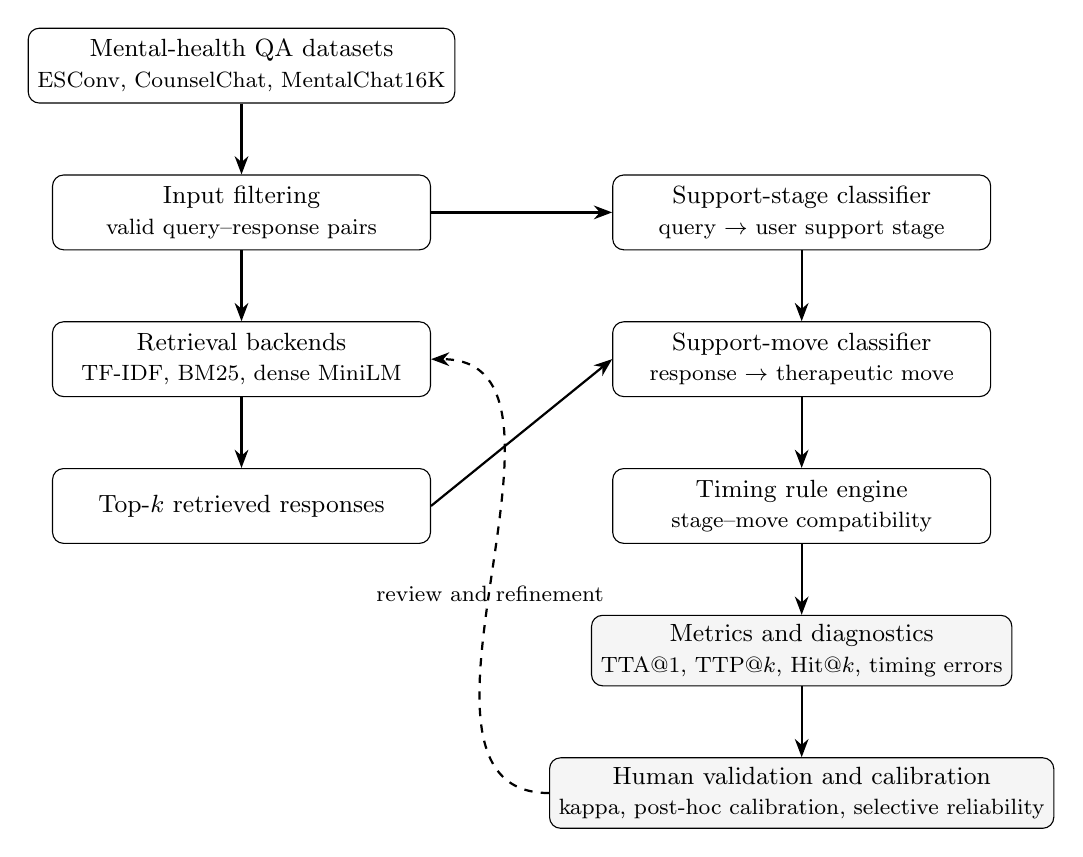
\begin{tikzpicture}[
    node distance=0.9cm,
    box/.style={
        rectangle,
        rounded corners=4pt,
        draw=black,
        align=center,
        minimum width=4.8cm,
        minimum height=0.95cm,
        fill=white,
        font=\small
    },
    smallbox/.style={
        rectangle,
        rounded corners=4pt,
        draw=black,
        align=center,
        minimum width=4.8cm,
        minimum height=0.85cm,
        fill=rowgray,
        font=\small
    },
    arrow/.style={-Stealth, thick},
    dashedarrow/.style={-Stealth, thick, dashed}
]

\node[box] (data) {Mental-health QA datasets\\
\footnotesize ESConv, CounselChat, MentalChat16K};

\node[box, below=of data] (filter) {Input filtering\\
\footnotesize valid query--response pairs};

\node[box, below=of filter] (retrieval) {Retrieval backends\\
\footnotesize TF-IDF, BM25, dense MiniLM};

\node[box, below=of retrieval] (candidates) {Top-\(k\) retrieved responses};

\node[box, right=2.3cm of filter] (stage) {Support-stage classifier\\
\footnotesize query \(\rightarrow\) user support stage};

\node[box, below=of stage] (move) {Support-move classifier\\
\footnotesize response \(\rightarrow\) therapeutic move};

\node[box, below=of move] (timing) {Timing rule engine\\
\footnotesize stage--move compatibility};

\node[smallbox, below=of timing] (metrics) {Metrics and diagnostics\\
\footnotesize TTA@1, TTP@\(k\), Hit@\(k\), timing errors};

\node[smallbox, below=of metrics] (calibration) {Human validation and calibration\\
\footnotesize kappa, post-hoc calibration, selective reliability};

\draw[arrow] (data) -- (filter);
\draw[arrow] (filter) -- (retrieval);
\draw[arrow] (retrieval) -- (candidates);

\draw[arrow] (filter.east) -- (stage.west);
\draw[arrow] (candidates.east) -- (move.west);

\draw[arrow] (stage) -- (move);
\draw[arrow] (move) -- (timing);
\draw[arrow] (timing) -- (metrics);
\draw[arrow] (metrics) -- (calibration);

\draw[dashedarrow] (calibration.west) to[out=180,in=0] node[below, font=\footnotesize] {review and refinement} (retrieval.east);

\end{tikzpicture}%
}
\caption{Overview of the TheraTime software framework. The left column shows data preparation and retrieval, while the right column shows therapeutic timing evaluation, diagnostics, human validation, and reliability-aware calibration.}
\label{fig:framework_overview}
\end{figure}

\subsection{Input filtering and datasets}
\label{subsec:datasets}

TheraTime operates on query-response pairs. Each input pair is filtered to remove greetings, fragments, very short responses, unusually long queries, and obvious non-informative artifacts. This reduces noise before retrieval and timing evaluation.

The illustrative experiment uses three public mental-health or emotional-support resources:

\begin{itemize}
    \item \textbf{ESConv.} A dataset of emotional support conversations designed around support strategies and help-seeker/supporter interactions~\cite{Liu2021ESConv}.
    \item \textbf{CounselChat.} A question-answer dataset derived from public counseling questions and therapist responses~\cite{Bertagnolli2018CounselChat}.
    \item \textbf{MentalChat16K.} A mental-health conversational assistance benchmark combining real anonymized interview data and synthetic dialogue data~\cite{Xu2025MentalChat16K}.
\end{itemize}

For each dataset, extraction stopped once the fixed cap of 800 valid pairs had been collected. The retrieval stage used up to 250 queries per dataset and per retrieval method, yielding 750 examples for each retrieval backend and 2250 query-level examples in total. Table~\ref{tab:dataset_construction} summarizes the dataset construction protocol used in the illustrative experiment.

\begin{table}[!htbp]
\centering
\caption{Dataset construction protocol for the illustrative experiment. The first column reports the extraction budget used by the released script rather than the full size of each public dataset.}
\label{tab:dataset_construction}
\small
\setlength{\tabcolsep}{5pt}
\renewcommand{\arraystretch}{1.15}
\rowcolors{2}{rowgray}{white}
\begin{tabularx}{\linewidth}{lcm{1.5cm}m{1.5cm}X}
\toprule
\textbf{Dataset} & \textbf{Rows inspected} & \textbf{Valid pairs kept} & \textbf{Queries used} & \textbf{Notes} \\
\midrule
ESConv & 300 conversation rows & 800 & 250 & Consecutive seeker--supporter turns were extracted after filtering. \\
CounselChat & Up to 1600 rows & 800 & 250 & Public counseling question--answer pairs were filtered for valid text length. \\
MentalChat16K & Up to 1600 rows & 800 & 250 & Conversational assistance examples were filtered into query--response pairs. \\
\midrule
Total & -- & 2400 & 750 per retrieval method & Each query was evaluated with top-\(k=5\) retrieved responses. \\
\bottomrule
\end{tabularx}
\end{table}

\subsection{Support-stage and support-move taxonomies}

TheraTime defines seven user support stages and nine response support moves (Tables~\ref{tab:stages} and~\ref{tab:moves}). The stages are intended to represent the user's current need, while the moves represent what the response is doing.

The taxonomy is not intended to replace clinical assessment. It is a lightweight operational taxonomy for retrieval evaluation. Its support-move categories are grounded in established counseling and dialogue-analysis ideas: Stiles' Verbal Response Mode framework distinguishes response functions such as disclosure, advisement, interpretation, reflection, and acknowledgment, while motivational interviewing emphasizes the timing of empathic listening, clarification, elicitation, and advice within client-centered support~\cite{Stiles1992VRM,Miller2013MI}. TheraTime adapts these ideas to an offline retrieval setting by representing user need as a support stage and response behavior as a support move, then evaluating whether the two are compatible.

\begin{table}[!htbp]
\centering
\small
\caption{TheraTime support-stage taxonomy.}
\label{tab:stages}
\rowcolors{2}{rowgray}{white}
\setlength{\tabcolsep}{5pt}
\renewcommand{\arraystretch}{1.15}
\begin{tabularx}{\linewidth}{p{3.8cm}X}
\toprule
\textbf{Stage} & \textbf{Meaning} \\
\midrule
distress\_disclosure & The user shares sadness, fear, loneliness, pain, or distress without yet asking for concrete help. \\
high\_emotional\_intensity & The user is overwhelmed, panicking, crying, spiraling, or emotionally dysregulated. \\
unclear\_need & The user is vague, confused, or unable to explain what is wrong. \\
advice\_seeking & The user explicitly asks for steps, strategies, coping techniques, or concrete actions. \\
psychoeducation\_seeking & The user asks why something is happening or requests an explanation. \\
crisis\_safety & The user states suicidal thoughts, self-harm intent, inability to stay safe, or urgent safety risk. \\
followup\_problem\_solving & The user has already received support and is now asking for planning or next steps. \\
\bottomrule
\end{tabularx}
\end{table}

\begin{table}[!htbp]
\centering
\small
\caption{TheraTime support-move taxonomy.}
\label{tab:moves}
\rowcolors{2}{rowgray}{white}
\setlength{\tabcolsep}{5pt}
\renewcommand{\arraystretch}{1.15}
\begin{tabularx}{\linewidth}{p{3.8cm}X}
\toprule
\textbf{Move} & \textbf{Meaning} \\
\midrule
validation & Acknowledges the user's feelings as understandable or valid. \\
empathy & Expresses warmth, care, and emotional presence. \\
reflective\_listening & Restates or mirrors the user's situation or feelings. \\
clarification & Asks a gentle question to better understand the user's need. \\
grounding & Helps the user calm down, breathe, stabilize, or focus on the present. \\
practical\_advice & Provides concrete coping steps, behavioral strategies, or action plans. \\
psychoeducation & Explains symptoms, emotional processes, or why feelings occur. \\
encouragement & Offers hope, reassurance, motivation, or affirmation. \\
safety\_referral & Directs the user toward emergency help, crisis support, a trusted person, or urgent safety resources. \\
\bottomrule
\end{tabularx}
\end{table}

\subsection{Prototype classifiers}

The timing module uses two prototype classifiers. The stage classifier maps the user query to one of the support stages. The move classifier maps the retrieved response to one of the support moves. Each label is represented by a short natural-language description. A sentence-transformer encoder embeds the input and the prototypes, and cosine similarity determines the predicted label.

The default timing encoder is \texttt{sentence-transformers/paraphrase-mpnet-base-v2}. Dense retrieval uses \texttt{sentence-transformers/all-MiniLM-L6-v2}. This separation is intentional: the retrieval model and the timing evaluator do not rely on the same default encoder, reducing circular bias between response selection and response assessment. Sentence-transformers are widely used to encode sentences into dense vectors for similarity and semantic search tasks~\cite{Reimers2019SentenceBERT}.

\subsection{Timing rule engine}
\label{subsec:timing_rule_engine}

Given a predicted stage \(s\) and a predicted move \(m\), TheraTime assigns a timing label using a rule-based compatibility table. The possible timing labels are:

\begin{itemize}
    \item \textbf{well\_timed}: the support move is compatible with the user's current support stage.
    \item \textbf{premature\_advice}: practical advice is given before validation, grounding, or clarification.
    \item \textbf{delayed\_safety}: safety risk is present but the response does not prioritize safety.
    \item \textbf{over\_validation}: the user asks for practical help but the response only validates, empathizes, or reflects.
    \item \textbf{missing\_clarification}: the user need is unclear but the response does not clarify.
    \item \textbf{stage\_mismatch}: the response move is incompatible with the predicted stage.
\end{itemize}

The core logic is transparent. For example, if \(s=\texttt{crisis\_safety}\) and \(m\notin\{\texttt{safety\_referral},\texttt{grounding},\texttt{validation}\}\), the timing label is \texttt{delayed\_safety}. If \(s=\texttt{unclear\_need}\) and the response gives practical advice instead of clarification or supportive presence, the label is \texttt{premature\_advice} or \texttt{missing\_clarification}, depending on the predicted move.

\subsection{Metrics and outputs}
\label{subsec:metrics}

TheraTime reports the following main metrics:

\begin{itemize}
    \item \textbf{TTA@1}: top-1 automatic well-timed rate, defined as the proportion of rank-1 retrieved responses assigned \texttt{well\_timed} by the automatic timing evaluator. This corpus-level metric is distinct from human-validated timing-label accuracy.
    \item \textbf{TTP@\(k\)}: automatic well-timed proportion over the top \(k\) retrieved responses, defined as the mean automatic \texttt{well\_timed} rate across rank \(\leq k\).
    \item \textbf{Hit@\(k\)}: the proportion of queries for which at least one response in the top \(k\) is well-timed.
    \item \textbf{Timing error rates}: rates of \texttt{premature\_advice}, \texttt{delayed\_safety}, \texttt{over\_validation}, \texttt{missing\_clarification}, and \texttt{stage\_mismatch}.
    \item \textbf{Confidence diagnostics}: stage and move prototype margins, low-confidence flags, and entropy over prototype scores.
\end{itemize}

The framework exports CSV and JSON outputs, including all automatic judgments, method-level comparison tables, ablation tables, design-verification outputs, diagnostic reports, annotation files, inter-annotator agreement reports, post-calibration outputs, selective reliability tables, and publication-ready figures.

\section{Human validation and reliability safeguards}
\label{sec:human_calibration}

\subsection{Human annotation protocol}

Human validation was conducted in two stages with different purposes. The first stage used 150 rank-1 examples assessed independently by two co-author annotators and served as an exploratory evaluation of taxonomy interpretability, inter-annotator agreement, and common correction patterns. The exploratory 150-example stage informed the design of the annotation protocol and taxonomy. The second stage used 300 rank-1 judgments and added a third annotator external to the author team. This larger three-annotator study constitutes the primary human-validation reference. All calibration results reported in this paper are based on the primary 300-example study, evaluated out of fold.

All annotators used the same fixed interface and predefined stage, move, and timing taxonomies. For each example, they answered three questions:

\begin{enumerate}
    \item Is the predicted support stage correct for the user query?
    \item Is the predicted support move correct for the retrieved response?
    \item Is the automatic final timing label correct for the query--response pair?
\end{enumerate}

Annotators selected \texttt{yes}, \texttt{no}, or \texttt{unsure}. When rejecting an automatic label, they could provide a corrected label and optional explanatory notes. In the three-annotator study, majority consensus was used as the primary reference. Missing or unsure votes were not counted as positive or negative votes. Cases in which a majority rejected the automatic timing label but no unique replacement label could be established remained in the overall accuracy denominator and were conservatively scored as incorrect.

The 150-example stage was used only to examine annotation feasibility and common correction patterns. It is not used for the formal calibration claims. To reduce optimistic bias, calibration on the 300-example study was evaluated using pooled five-fold out-of-fold predictions, with correction rules learned only from the training folds and each annotated example evaluated once as held-out data. The out-of-fold analysis is included as a validity safeguard rather than as a separate contribution.

Although the dedicated error-recall utility originated during the earlier two-annotator pilot, the released notebook also applies it to selected annotator pairs within the 300-example study as an exploratory diagnostic. These pairwise analyses use only the two selected annotation files and the disagreement subset generated by the kappa utility; they do not replace the three-annotator majority reference.

\subsection{Consensus construction and agreement}

For each annotation target, a majority vote determined whether the automatic label was accepted or rejected. A correction was retained only when the required majority supplied the same valid replacement label. Conservative rules required stronger support and correction agreement. In nine timing cases, the majority rejected the automatic label but distinct valid replacement labels tied in vote count, so no unique majority replacement could be determined. These cases were retained in the 300-example denominator and scored as incorrect. Annotation identifiers were matched exactly against unique rank-1 automatic-judgment identifiers; missing or duplicated identifiers caused the calibration procedure to stop rather than silently reducing the evaluation sample.

Pairwise Cohen's kappa was used to quantify agreement between annotator pairs~\cite{Cohen1960Kappa}, with conventional descriptive ranges interpreted cautiously~\cite{Landis1977Kappa}. To separate annotation roles from author identities in reporting, the two co-author annotators are denoted \emph{Internal~1} and \emph{Internal~2}, while the third annotator is denoted \emph{External}. Agreement with the external annotator remained substantial for stage, move, and timing judgments, although move agreement was lower than between the two co-author annotators (Table~\ref{tab:pairwise_kappa}). This reduces concern that the consensus merely reflects shared author expectations, but it does not replace future validation by a larger independent clinical or professionally trained panel.

\begin{table}[!htbp]
\centering
\caption{Pairwise Cohen's kappa for the primary 300-example, three-annotator validation study.}
\label{tab:pairwise_kappa}
\small
\setlength{\tabcolsep}{6pt}
\renewcommand{\arraystretch}{1.15}
\rowcolors{2}{rowgray}{white}
\begin{tabular}{lccc}
\toprule
\textbf{Question} &
\textbf{Internal 1--Internal 2} &
\textbf{Internal 1--External} &
\textbf{Internal 2--External} \\
\midrule
Stage correctness  & 0.624 & 0.671 & 0.730 \\
Move correctness   & 0.851 & 0.634 & 0.638 \\
Timing correctness & 0.733 & 0.647 & 0.687 \\
\bottomrule
\end{tabular}
\end{table}

\subsection{Human-validated automatic-label accuracy}

The two annotation stages used different panel sizes and consensus criteria. In the exploratory two-annotator stage, both annotators accepted the automatic timing label in 34 of 150 cases (22.7\%) under a strict joint-acceptance criterion. In the primary three-annotator study, the automatic timing label was accepted in 151 of 300 cases (50.3\%) under majority consensus and in 108 of 300 cases (36.0\%) under the stricter all-three-agree criterion. These values are not directly interchangeable. The three-annotator majority-consensus labels are used as the reference for the subsequent calibration analyses.

The component labels also remained noisy. Under all-three agreement, the automatic stage and move labels were each accepted in 25.7\% of examples. Under majority consensus, the corresponding rates were 39.3\% for stage and 36.7\% for move (Table~\ref{tab:auto_label_accuracy_300}). These results support using TheraTime for screening, diagnostic analysis, and human-review support rather than as a final automatic timing judge.

\begin{table}[!htbp]
\centering
\caption{Automatic-label acceptance in the primary 300-example annotation study. Strict agreement requires all three annotators to accept the automatic label; majority agreement requires at least two of three.}
\label{tab:auto_label_accuracy_300}
\small
\rowcolors{2}{rowgray}{white}
\begin{tabular}{lcc}
\toprule
\textbf{Automatic label} &
\textbf{Strict all-agree} &
\textbf{Majority consensus} \\
\midrule
Stage  & 25.7\% & 39.3\% \\
Move   & 25.7\% & 36.7\% \\
Timing & 36.0\% & 50.3\% \\
\bottomrule
\end{tabular}
\end{table}

\subsection{Correction-direction analysis}

Both annotation stages showed the same dominant correction pattern: automatic timing warnings were frequently corrected to \texttt{well\_timed}. Among 120 examples in which the majority rejected the automatic timing label and a valid consensus correction was available, 112 cases (93.3\%) were corrected to \texttt{well\_timed}. Only eight cases (6.7\%) remained mistimed under a different error subtype (Table~\ref{tab:correction_direction_300}). This result provides direct quantitative evidence that the current timing engine is more suitable for screening candidate concerns than for issuing final automatic judgments.

\begin{table}[!htbp]
\centering
\caption{Correction direction for rejected automatic timing labels with a valid majority-consensus replacement in the primary 300-example study.}
\label{tab:correction_direction_300}
\small
\rowcolors{2}{rowgray}{white}
\begin{tabular}{lrr}
\toprule
\textbf{Human correction direction} & \textbf{Count} & \textbf{Proportion} \\
\midrule
Corrected to \texttt{well\_timed} & 112 & 93.3\% \\
Still mistimed with a different subtype & 8 & 6.7\% \\
\midrule
Total valid corrections & 120 & 100.0\% \\
\bottomrule
\end{tabular}
\end{table}

As a secondary diagnostic, pairwise analyses of selected annotator combinations showed the same dominant pattern of conservative over-flagging, with most jointly rejected automatic timing warnings corrected to \texttt{well\_timed}. These pairwise results are provided in the released notebook and are not used in the primary three-annotator majority-consensus or pooled calibration analyses.

The exploratory annotation stage is retained to document the development of the validation protocol, but its descriptive post-hoc calibration results are not used as formal evidence in this paper.

\subsection{Qualitative examples of system behaviour}
\label{subsec:qualitative_examples}

Table~\ref{tab:qualitative_examples} presents seven representative cases from the primary three-annotator study. The examples include correct well-timed judgments, correctly detected safety-related timing errors, false-positive warnings, a wrong error subtype, and a case without timing consensus. Predicted stage and move labels are shown alongside the corresponding human labels to make clear whether component-level agreement affected the final timing judgment. Query and response excerpts are shortened only for presentation; the released example file retains the complete records and identifiers.

\begin{table*}[!htbp]
\centering
\caption{Representative examples from the primary three-annotator study. ``No majority'' indicates that no stage or timing label obtained the required annotator majority.}
\label{tab:qualitative_examples}
\scriptsize
\setlength{\tabcolsep}{2.4pt}
\renewcommand{\arraystretch}{1.13}
\rowcolors{2}{rowgray}{white}
\resizebox{\textwidth}{!}{%
\begin{tabular}{c p{2.7cm} p{3.3cm} p{2.5cm} p{2.2cm} p{2.2cm} p{2.2cm} p{2.1cm} p{2.1cm} p{2.1cm} p{4.2cm}}
\toprule
\textbf{Ex.} &
\textbf{Query excerpt} &
\textbf{Response excerpt} &
\textbf{Predicted stage} &
\textbf{Predicted move} &
\textbf{Automatic timing} &
\textbf{Human stage} &
\textbf{Human move} &
\textbf{Human timing} &
\textbf{Case type} &
\textbf{Interpretation} \\
\midrule
1 &
The user says breathing exercises would be helpful. &
The response encourages trying breathing exercises. &
\texttt{high\_emotional\_intensity} &
\texttt{grounding} &
\texttt{well\_timed} &
\texttt{distress\_disclosure} &
\texttt{grounding} &
\texttt{well\_timed} &
Correct timing &
All three annotators accepted the final timing judgment, although the majority assigned a different support stage. \\

2 &
The user describes anxiety linked to perfectionism and fear of mistakes. &
The response validates disappointment and frames mistakes as part of human experience. &
\texttt{psychoeducation\_seeking} &
\texttt{clarification} &
\texttt{well\_timed} &
\texttt{distress\_disclosure} &
\texttt{validation} &
\texttt{well\_timed} &
Correct timing &
All three accepted the final timing judgment, although the majority assigned different stage and move labels. \\

3 &
The user reports recent self-harm and recurrent urges under stress (retrieved response A). &
The response questions the diagnostic labels and suggests seeking another opinion. &
\texttt{crisis\_safety} &
\texttt{psychoeducation} &
\texttt{delayed\_safety} &
\texttt{crisis\_safety} &
\texttt{practical\_advice} &
\texttt{delayed\_safety} &
Correct warning &
The safety warning remained stable despite disagreement about the exact response move. \\

4 &
The user reports recent self-harm and recurrent urges under stress (retrieved response B). &
The response explains self-harm as a learned coping pattern without foregrounding immediate safety action. &
\texttt{crisis\_safety} &
\texttt{practical\_advice} &
\texttt{delayed\_safety} &
\texttt{crisis\_safety} &
\texttt{empathy} &
\texttt{delayed\_safety} &
Correct warning &
All three annotators accepted the delayed-safety judgment despite move-level disagreement. \\

5 &
The user describes concern about risks to self and family. &
The response validates stress, fear, and concern about family illness. &
\texttt{advice\_seeking} &
\texttt{clarification} &
\texttt{stage\_mismatch} &
No majority &
\texttt{empathy} &
\texttt{well\_timed} &
False positive &
All three rejected the timing-error label and judged the response well timed; no majority stage label was established. \\

6 &
The user describes chronic illness, loneliness, and asks how to cope. &
The response emphasizes that progress on one issue may improve overall well-being. &
\texttt{distress\_disclosure} &
\texttt{practical\_advice} &
\texttt{premature\_advice} &
\texttt{advice\_seeking} &
\texttt{empathy} &
\texttt{over\_validation} &
Wrong subtype &
The system detected a timing concern, but disagreement in both component labels produced the wrong error subtype. \\

7 &
The user reports anxiety, depression, missed deadlines, and panic attacks at work. &
The response acknowledges distress and suggests exploring support options. &
\texttt{advice\_seeking} &
\texttt{practical\_advice} &
\texttt{well\_timed} &
\texttt{high\_emotional\_intensity} &
\texttt{practical\_advice} &
No majority &
Boundary case &
No timing label obtained the required majority, illustrating a judgment boundary under the fixed taxonomy. \\
\bottomrule
\end{tabular}}
\end{table*}

These examples show that correct final timing judgments can occur despite disagreement about stage or move, while component errors can also produce false-positive warnings or the wrong timing subtype. They support the use of TheraTime as an inspectable screening and analysis framework rather than as a final automatic therapeutic judge.

\FloatBarrier

\subsection{Primary validation-gated calibration on 300 examples}

The primary 300-example calibration used three-annotator majority-consensus labels and was evaluated using pooled five-fold out-of-fold predictions to avoid testing correction rules on the same examples from which they were learned. Within each fold, candidate stage--move correction rules were derived from the training folds and screened on an inner validation subset using a do-no-harm criterion: a rule was retained only when it affected a minimum number of validation examples, improved timing-label accuracy, and did not reduce balanced accuracy. Each of the 300 annotated examples therefore contributed once to the final evaluation as unseen held-out data.

In the pooled evaluation, the uncalibrated baseline achieved a timing-label accuracy of 0.5033 (95\% bootstrap CI 0.4467--0.5633). Conservative stage--move recomputation produced the same pooled accuracy. The validation-gated correction policy achieved 0.6167 (95\% CI 0.5600--0.6700), corresponding to an absolute gain of 0.1133. A paired bootstrap over the same held-out predictions yielded a 95\% confidence interval of 0.0767--0.1500 for the gain (Table~\ref{tab:calibration}). The out-of-fold analysis is reported to reduce in-sample calibration bias; it does not remove the limitations associated with the moderate annotation sample or establish external clinical validity.

\begin{table}[!htbp]
\centering
\caption{Primary five-fold pooled out-of-fold timing-label accuracy on all 300 human-validated examples.}
\label{tab:calibration}
\small
\setlength{\tabcolsep}{5pt}
\renewcommand{\arraystretch}{1.15}
\rowcolors{2}{rowgray}{white}
\begin{tabularx}{\linewidth}{lccc}
\toprule
\textbf{Method} &
\textbf{Pooled accuracy} &
\textbf{95\% CI} &
\textbf{Gain vs. baseline} \\
\midrule
Baseline &
0.5033 &
0.4467--0.5633 &
0.0000 \\
Conservative stage--move recomputation &
0.5033 &
0.4467--0.5633 &
0.0000 \\
Validation-gated correction policy &
\best{0.6167} &
0.5600--0.6700 &
\best{+0.1133} \\
\bottomrule
\end{tabularx}
\end{table}

The paired-bootstrap 95\% confidence interval for the validation-gated policy's improvement over baseline was 0.0767--0.1500. Because this interval excludes zero, the pooled gain is statistically significant at the 0.05 level.

\subsection{Selective reliability analysis}
\label{subsec:selective_reliability}

TheraTime also retains selective reliability analysis as a secondary diagnostic. Post-hoc calibration and confidence estimation are used to distinguish higher-confidence cases from cases requiring review, following established calibration and risk--coverage principles~\cite{Guo2017Calibration,Geifman2019SelectiveNet}. In a complementary 70/30 held-out analysis, the restrictive validation-gated policy accepted 19 of 90 cases (21.1\% coverage), of which 18 agreed with the human-majority timing label (94.7\% accepted-subset accuracy); the remaining 71 cases were referred for review. Across ten repeated development--held-out splits, the policy achieved a mean accuracy of 0.6678 with a standard deviation of 0.0855 and a range of 0.5000--0.8111, indicating a positive average effect together with meaningful split sensitivity. A threshold sensitivity check showed the expected trade-off: less restrictive thresholds increased coverage but reduced accepted-subset accuracy. These analyses are reported to characterize the operating behaviour of the framework, not as primary performance claims; the pooled five-fold out-of-fold comparison over all 300 annotated examples remains the main calibration result.

\FloatBarrier

\section{Software metadata, availability, and versioning}
\label{sec:availability}

\subsection{Repository and license}

The current implementation is a Python research framework developed for offline experiments in notebook and script environments. It consists of the following modules:

\begin{itemize}
    \item \texttt{theratime\_v06\_neurocomputing.py}: main retrieval and timing-evaluation pipeline for dataset loading, retrieval, stage classification, move classification, rule-based timing assessment, metrics, and output generation.
    \item \texttt{annotations/}: repository folder containing the three completed 300-example annotation CSV files used in the primary human-validation analysis, together with a blank annotation template that can be reused for new annotation studies.
    \item \texttt{theratime\_kappa.py}: pairwise Cohen's-kappa utility for exactly two annotation files. To reproduce the three pairwise results in Table~\ref{tab:pairwise_kappa}, the utility is run once for each annotator pair.
    \item \texttt{theratime\_post\_calibration.py}: reusable calibration library providing annotation loading, majority-consensus construction, held-out splitting, do-no-harm rule learning, correction-rule evaluation, and keep/correct/review policy functions. It has no command-line interface and is imported by \texttt{theratime\_calibration\_robustness.py}.
    \item \texttt{theratime\_calibration\_robustness.py}: command-line driver for the primary 300-example calibration analysis, including bootstrap confidence intervals, ten-seed repeated-split stability, threshold sensitivity, reliability diagnostics, rank-based coverage, pooled five-fold out-of-fold evaluation, and paired significance testing.
    \item \texttt{theratime\_selective\_reliability.py}: legacy descriptive risk--coverage utility retained as a secondary diagnostic; it is not used for the primary human-validated accuracy claim.
    \item \texttt{theratime\_error\_recall.py}: exploratory pairwise correction-analysis utility for selected annotator pairs. Its outputs are secondary diagnostics and are not used to compute the primary three-annotator majority-consensus or pooled calibration results.
    \item \texttt{notebooks/theratime.ipynb}: released notebook used to execute the documented Kaggle analysis workflow and generate the reported diagnostic outputs.
\end{itemize}

The software is available at \theratimeRepository{} and the archived release is available through Zenodo at \theratimeZenodo{}. Executable examples matching the released notebook are provided in \texttt{examples/example\_kaggle\_commands.md}. The repository includes an \texttt{annotations/} folder containing the three completed 300-example annotation files corresponding to Internal~1, Internal~2, and External, as well as a blank CSV template with the same schema. Users may reproduce the reported analyses directly from the released annotation files or apply the template to new examples and annotators. The illustrative retrieval experiment uses the public ESConv, CounselChat, and MentalChat16K datasets, subject to their original licenses. The three 300-example annotation files used for pairwise agreement, majority-consensus construction, and calibration are included in the repository's \texttt{annotations/} folder, together with a reusable blank template. The recommended license is the MIT License for the software code. Dataset-specific licenses and terms must be respected separately.

\subsection{Software metadata}

Table~\ref{tab:metadata} summarises the main software metadata. The implementation relies on scikit-learn for TF-IDF and statistical utilities, Hugging Face Datasets for dataset access, and the broader Transformer software ecosystem used by sentence-transformer encoders~\cite{Pedregosa2011ScikitLearn,McInnes2021HuggingFaceDatasets,Wolf2020Transformers}.

\begin{table}
\centering
\footnotesize
\caption{Software metadata for TheraTime.}
\label{tab:metadata}
\rowcolors{2}{rowgray}{white}
\setlength{\tabcolsep}{6pt}
\renewcommand{\arraystretch}{1.2}
\begin{tabular}{p{3.7cm} p{8.2cm}}
\toprule
Item & Description \\
\midrule
Software name & TheraTime \\
Repository & \theratimeRepository{} \\
Archived release & \theratimeZenodo{} \\
Current version & v1.0.0 \\
Software type & Offline research evaluation framework \\
Programming language & Python \\
Core dependencies & pandas, NumPy, SciPy, scikit-learn, matplotlib, datasets, sentence-transformers, rank-bm25, tqdm, openpyxl \\
Supported environment & Kaggle, Linux, local Python environments with CPU or GPU support \\
Default timing encoder & \texttt{sentence-transformers/paraphrase-mpnet-base-v2} \\
Dense retrieval encoder & \texttt{sentence-transformers/all-MiniLM-L6-v2} \\
Retrieval backends & TF-IDF, BM25, dense MiniLM retrieval \\
Main outputs & CSV and JSON reports, diagnostic tables, annotation files, held-out calibration outputs, robustness reports, confidence intervals, threshold sensitivity, and risk--coverage analysis \\
Responsible-use status & Offline research evaluation only, not clinical decision support \\
\bottomrule
\end{tabular}
\end{table}

\FloatBarrier


\subsection{Reproducing the human-validation analyses}

The primary calibration workflow is executed through
\texttt{theratime\_calibration\_robustness.py}, using the rank-1 automatic
judgment file \texttt{all\_judgments\_mpnet.csv} and the three annotation
files \texttt{annotations/theratime\_annotation\_sample\_300\_internal1.csv},
\texttt{annotations/theratime\_annotation\_sample\_300\_internal2.csv}, and
\texttt{annotations/theratime\_annotation\_sample\_300\_external.csv}. The driver imports the reusable
consensus and calibration functions from
\texttt{theratime\_post\_calibration.py}.

The blank annotation template follows the same schema expected by the analysis scripts, including example identifiers, query and response text, automatic stage, move, and timing labels, correctness judgments, optional correction fields, notes, and an annotator field. The reusable blank template is stored as \texttt{annotations/theratime\_annotation\_template.csv}. Its exported outputs include
\texttt{theratime\_bootstrap\_ci.csv},
\texttt{theratime\_multiseed\_per\_seed.csv},
\texttt{theratime\_multiseed\_aggregate.csv},
\texttt{theratime\_threshold\_sweep.csv},
\texttt{theratime\_reliability\_diagnostics.csv},
\texttt{theratime\_coverage\_target\_report.csv},
\texttt{theratime\_kfold\_pooled\_summary.csv},
method-specific pooled prediction files, and
\texttt{theratime\_paired\_significance.csv}.

The correction-direction result in Table~\ref{tab:correction_direction_300}
is computed from the same three-annotator majority-consensus output produced
by \texttt{build\_consensus()} in
\texttt{theratime\_post\_calibration.py}. For this direction-specific
summary, majority-rejected cases are included only when a valid non-tied
replacement differs from the automatic timing label. Correction ties and
cases without a valid shared replacement are excluded from the
direction-specific denominator, but all rejected cases remain errors in the
overall 300-example automatic-label accuracy denominator. The accompanying
README provides the exact reproduction snippet.

Pairwise agreement is reproduced by running
\texttt{theratime\_kappa.py} three times: Internal~1--Internal~2,
Internal~1--External, and Internal~2--External. The \texttt{theratime\_error\_recall.py} utility is used only for secondary
pairwise diagnostics on selected annotator pairs. It analyzes the disagreement
CSV produced by \texttt{theratime\_kappa.py} together with the corresponding
full annotation files. Its disagreement-subset correction rates and strict
pairwise confirmation rates are not used to construct the primary
three-annotator majority-consensus reference and do not contribute to the
pooled five-fold calibration result.

\subsection{Versioning and maintenance}

The code version associated with this paper is v1.0.0. Future releases should follow semantic versioning. Minor versions may add new taxonomies, datasets, retrieval methods, or calibration strategies. Major versions should be reserved for changes that alter the public output schema or the meaning of timing labels.

\FloatBarrier

\section{Illustrative example: therapeutic timing evaluation across three datasets}
\label{sec:example}

\subsection{Experimental setup}

The illustrative experiment used ESConv, CounselChat, and MentalChat16K. For each dataset, 800 valid query-response pairs were extracted. For each retrieval method, the first 250 valid queries per dataset were used, yielding 750 examples for TF-IDF, 750 for BM25, and 750 for dense MiniLM retrieval. Each query was evaluated with top-\(k=5\) retrieved responses, producing 11250 ranked timing judgments.

The default timing system used MPNet prototype classifiers for both stage and move prediction. Two ablations were also evaluated: a MiniLM timing encoder ablation and a keyword-stage ablation with MPNet move classification.

\subsection{Primary retrieval comparison}

Table~\ref{tab:retrieval_results} reports the primary method comparison. BM25 produced the highest top-1 automatic well-timed rate, followed by TF-IDF. Dense MiniLM retrieval had the lowest TTA@1 and the highest stage-mismatch rate.

\begin{table*}[!htbp]
\centering
\caption{Primary retrieval comparison under the default MPNet timing evaluator.}
\label{tab:retrieval_results}
\resizebox{\linewidth}{!}{%
\rowcolors{2}{rowgray}{white}
\begin{tabular}{lrrrrrr}
\toprule
\textbf{Retrieval method} & \textbf{TTA@1} & \textbf{95\% CI low} & \textbf{95\% CI high} & \textbf{TTP@5} & \textbf{Hit@5} & \textbf{Stage-mismatch rate} \\
\midrule
TF-IDF & 0.5760 & 0.5413 & 0.6120 & 0.5331 & 0.9107 & 0.2987 \\
BM25 & \best{0.6053} & 0.5707 & 0.6413 & 0.5341 & \best{0.9240} & 0.2453 \\
Dense MiniLM & 0.4187 & 0.3840 & 0.4533 & 0.4901 & 0.8933 & 0.4400 \\
\bottomrule
\end{tabular}}
\end{table*}

The result suggests that semantic dense retrieval does not automatically produce better therapeutic timing. Lexical retrieval methods, especially BM25, retrieved more well-timed top-ranked responses in this setting. This supports the central motivation of TheraTime: retrieval similarity and therapeutic timing should be evaluated separately. The result is also consistent with recent healthcare retrieval-augmented generation discussions, which emphasize that retrieval can improve reliability only when retrieved content is appropriate, contextualized, and evaluated with domain-specific criteria rather than with generic relevance alone~\cite{Yang2025RAGHealthcare,Amugongo2025RAGHealthcareReview}. Figure~\ref{fig:retrieval_correlation} further shows that retrieval score has only a weak relationship with automatic timing, reinforcing the need for timing-specific evaluation rather than relying on retrieval score alone.

\begin{figure}[!htbp]
    \centering
    \includegraphics[width=0.92\linewidth]{retrieval_score_vs_timing_correlation.png}
    \caption{Point-biserial correlation between retrieval score and automatic therapeutic timing. Retrieval score is only weakly associated with timing correctness, supporting timing-specific evaluation instead of relying on generic retrieval confidence alone.}
    \label{fig:retrieval_correlation}
\end{figure}

\FloatBarrier

\subsection{Ablation study}

Table~\ref{tab:ablation} and Figure~\ref{fig:ablation_tta1} report the timing-system ablations. The MPNet default achieved the highest overall TTA@1, while the MiniLM timing encoder produced a lower TTA@1. The keyword-stage ablation reduced stage-mismatch rate but also lowered overall TTA@1 relative to MPNet, indicating that simple keyword staging is not sufficient. Paired McNemar tests on rank-1 timing decisions confirmed that the MPNet default differed significantly from the MiniLM timing ablation (\(\chi^2=97.7\)) and from the keyword-stage ablation (\(\chi^2=22.4\)); both comparisons were significant at \(p<0.05\)~\cite{McNemar1947}.

\begin{table*}[!htbp]
\centering
\caption{Ablation results across all retrieval methods.}
\label{tab:ablation}
\resizebox{\linewidth}{!}{%
\rowcolors{2}{rowgray}{white}
\begin{tabular}{lrrrrr}
\toprule
\textbf{Configuration} & \textbf{TTA@1} & \textbf{95\% CI low} & \textbf{95\% CI high} & \textbf{Stage-mismatch rate} & \textbf{Low-confidence rate} \\
\midrule
MPNet stage + MPNet move & \best{0.5333} & 0.5129 & 0.5542 & 0.3280 & 0.2422 \\
MiniLM stage + MiniLM move & 0.3898 & 0.3693 & 0.4102 & 0.4147 & 0.1920 \\
Keyword stage + MPNet move & 0.4564 & 0.4360 & 0.4769 & 0.0742 & 0.1649 \\
\bottomrule
\end{tabular}}
\end{table*}

\begin{figure}[!htbp]
    \centering
    \includegraphics[width=\linewidth]{ablation_tta1.png}
    \caption{Ablation comparison for top-1 automatic well-timed rate. The default MPNet stage and move classifiers obtain the highest TTA@1, while MiniLM timing and keyword-stage ablations reduce performance. Error bars denote 95\% bootstrap confidence intervals.}
    \label{fig:ablation_tta1}
\end{figure}

\subsection{Design verification controls}

The design verification controls contained five manually designed vignettes: premature advice, delayed safety, over-validation, missing clarification, and a positive distress-control case (Table~\ref{tab:stress}). These controls are not intended as clinical safety tests; they are sanity checks used to verify that the rule engine detects clear, deliberately constructed timing failures. The results matched the expected design: rank-1 responses were mistimed for the first four negative-control cases and well-timed for the positive-control case. The top-2 list always contained at least one well-timed response.

\begin{table}[!htbp]
\centering
\caption{Design verification summary.}
\label{tab:stress}
\rowcolors{2}{rowgray}{white}
\begin{tabular}{lr}
\toprule
\textbf{Metric} & \textbf{Value} \\
\midrule
TTA@1 & 0.20 \\
TTP@2 & 0.60 \\
Hit@2 & 1.00 \\
\bottomrule
\end{tabular}
\end{table}

The design verification controls show that the timing rule engine detects clear timing failures and can identify better alternatives within the retrieved list. They should not be interpreted as evidence of clinical robustness.

\subsection{Diagnostic visualisations}

TheraTime generates diagnostic plots to help interpret why retrieved responses are marked as well-timed or mistimed. Figure~\ref{fig:error_breakdown} shows the top-1 timing error composition for each retrieval method. Dense MiniLM produces the largest stage-mismatch component, consistent with its lower TTA@1. Figure~\ref{fig:move_distribution} shows that retrieved responses are dominated by clarification, practical advice, empathy, and grounding, while safety-referral and validation labels are comparatively rare. This imbalance helps explain why stage--move consistency remains low and why timing-aware evaluation is useful.

\begin{figure}[!htbp]
    \centering
    \includegraphics[width=0.95\linewidth]{error_breakdown.png}
    \caption{Top-1 timing error breakdown by retrieval method. Stage mismatch is the dominant error category, especially for dense MiniLM retrieval.}
    \label{fig:error_breakdown}
\end{figure}

\begin{figure}[!htbp]
    \centering
    \includegraphics[width=0.95\linewidth]{corpus_move_distribution.png}
    \caption{Predicted support-move distribution across retrieved responses. The response pool is dominated by clarification, practical advice, empathy, and grounding, while safety-referral and validation are rare.}
    \label{fig:move_distribution}
\end{figure}

Figure~\ref{fig:stage_distribution} compares predicted stage distributions between the neural stage classifier and the keyword-stage ablation. The keyword baseline collapses heavily toward \texttt{unclear\_need}, whereas the neural system distributes cases across advice seeking, distress disclosure, follow-up problem solving, psychoeducation seeking, and other stages. Figure~\ref{fig:confidence_distribution} shows the stage and move confidence-margin distributions and the adaptive confidence thresholds used for uncertainty flagging. The internal stage--move coherence diagnostic also showed low primary-move consistency (0.1902), indicating that the retrieved response pool often delivered moves that did not match the ideal primary move for the predicted stage. Finally, Figure~\ref{fig:geometry_entropy} plots retrieval score against stage-prototype entropy and shows that their joint geometry does not separate well-timed and mistimed cases cleanly. Separately, the global point-biserial correlation between retrieval score and the binary automatic timing label was small (\(r=0.1429\)). This pooled statistic differs from the method-specific correlations shown in Figure~\ref{fig:retrieval_correlation}, which are computed separately for TF--IDF, BM25, and dense MiniLM retrieval. Together, these analyses support treating geometry features as diagnostics rather than as clinical validation.

\begin{figure}[!htbp]
    \centering
    \includegraphics[width=0.95\linewidth]{stage_distribution_neural_vs_keyword.png}
    \caption{Predicted support-stage distribution for the neural stage classifier and keyword-stage ablation. The keyword baseline is dominated by \texttt{unclear\_need}, while the neural system produces a broader distribution of stages.}
    \label{fig:stage_distribution}
\end{figure}

\begin{figure*}[!htbp]
    \centering
    \includegraphics[width=\linewidth]{confidence_distributions.png}
    \caption{Stage and move confidence-margin distributions. The red dashed lines indicate adaptive p10 confidence-margin thresholds used to flag low-confidence timing judgments, matching the final v0.6 configuration.}
    \label{fig:confidence_distribution}
\end{figure*}

\begin{figure}[!htbp]
    \centering
    \includegraphics[width=0.95\linewidth]{geometry_retrieval_vs_stage_entropy.png}
    \caption{Retrieval score versus stage-prototype entropy for rank-1 judgments. The overlap between well-timed and mistimed cases shows that embedding geometry is diagnostic but not sufficient as a standalone validation signal. The narrow entropy range reflects the softmax normalization over seven stages with similar prototype distances, producing uniformly high entropy across the corpus.}
    \label{fig:geometry_entropy}
\end{figure}

\FloatBarrier

\section{Impact and reuse potential}
\label{sec:impact}

TheraTime has four main reuse scenarios.

\begin{itemize}
    \item \textbf{Retrieval benchmarking.} Researchers can compare response retrieval methods not only by semantic similarity, but also by timing appropriateness.
    \item \textbf{Error analysis.} The timing labels identify common failure modes, including premature advice, delayed safety, over-validation, missing clarification, and stage mismatch.
    \item \textbf{Human validation studies.} The released annotation CSV schema, blank template, completed annotation files, and kappa-analysis scripts support reproducible human-evaluation studies.
    \item \textbf{Reliability-aware evaluation.} The calibration and selective-reliability modules support cautious correction analysis and referral of uncertain cases for human review.
\end{itemize}

The main scientific contribution is not that TheraTime provides reliable final automatic judgments. Rather, the framework operationalizes therapeutic timing as a measurable retrieval property and provides transparent tools for evaluating, validating, and calibrating it. This is useful for building safer and more interpretable research pipelines in mental-health NLP.

\FloatBarrier

\section{Reproducibility and software quality assurance}
\label{sec:repro_qa}

\subsection{Reproducibility practices}

The experiment is reproducible through explicit software parameters and saved outputs:

\begin{itemize}
    \item Dataset names, retrieval encoders, timing encoders, top-\(k\), bootstrap settings, and random seed are defined at the top of the main script.
    \item The output directory stores all judgment tables, diagnostic reports, design-verification outputs, calibration files, and reproducibility metadata.
    \item Dense retrieval and default timing classification use different encoders by design.
    \item The 300-example human-validation set, five-fold assignments, inner validation splits, and random seeds are recorded in the calibration reports.
    \item Human annotation outputs are exported as CSV or JSON and can be re-analyzed for majority consensus, pairwise agreement, and out-of-fold calibration.
\end{itemize}

\subsection{Quality assurance}

TheraTime includes several quality controls:

\begin{itemize}
    \item \textbf{Input quality filter.} Short fragments, greetings, and non-informative cases are removed before evaluation.
    \item \textbf{Self-retrieval exclusion.} A query's original response is excluded from its retrieval pool to avoid trivial matches.
    \item \textbf{Design verification controls.} Hand-crafted vignettes verify that clear timing failures are detected.
    \item \textbf{Three-annotator consensus.} Majority consensus provides the human reference, while missing or unsure votes are not counted as valid positive or negative decisions.
    \item \textbf{Do-no-harm rule screening.} Candidate rules must improve inner-validation timing accuracy without reducing balanced accuracy before they can be applied.
    \item \textbf{Out-of-fold evaluation.} Calibration rules are learned only from training folds, and each annotated example is evaluated once as unseen held-out data. Bootstrap confidence intervals are reported for the pooled comparison.
\end{itemize}

\subsection{Responsible-use framing}

The recent literature increasingly emphasizes that mental-health LLM systems require rigorous safety, privacy, bias, and clinical evaluation before real-world use~\cite{Guo2024LLMMentalHealth,Hua2025ScopingLLMMentalHealth,Voultsiou2026LLMMentalHealth}. TheraTime therefore adopts a deliberately conservative framing. It evaluates retrieved responses offline, exposes timing errors, and flags uncertain cases for human review. It does not generate clinical advice, does not replace professional assessment, and does not provide crisis intervention.

\subsection{Limitations}

Several limitations should be noted.

\begin{itemize}
    \item \textbf{Prototype-label noise.} The stage and move classifiers are zero-shot prototype classifiers. They are interpretable and lightweight, but human validation shows that their raw labels remain noisy.
    \item \textbf{Annotator composition and external validity.} The primary study used two co-author annotators and one annotator external to the author team. Independent annotation, a fixed interface, predefined labels, and majority consensus reduce but do not eliminate familiarity or expectation bias. The panel should not be interpreted as clinical validation; larger studies involving independent clinicians, counselors, or trained mental-health annotators are needed before stronger safety or deployment claims can be made.
    \item \textbf{Human-validation scale.} The primary human-validation sample contains 300 examples. Five-fold pooling evaluates every example out of fold but does not create new independent data, so the resulting confidence intervals should not be interpreted as external-validation guarantees.
    \item \textbf{Selective reliability.} The complementary held-out policy accepted a limited subset of cases, and repeated-split results showed sensitivity to sample composition. These findings characterize a conservative review-oriented operating point rather than broad automatic coverage.
    \item \textbf{Offline evaluation only.} The framework evaluates timing categories, not clinical appropriateness in the full medical sense. It should not be used with real users or crisis situations without extensive clinical validation, governance, and safety procedures.
\end{itemize}

\FloatBarrier

\section{Conclusions}
\label{sec:conclusion}

This paper presented TheraTime, an offline software framework for therapeutic timing evaluation in mental-health response retrieval. The framework separates user support-stage classification, response support-move classification, and rule-based timing assessment. It evaluates multiple retrieval methods, reports timing-specific metrics and error categories, and includes design verification, human annotation, consensus construction, out-of-fold post-hoc calibration and selective human-review routing.

The illustrative retrieval experiment shows that therapeutic timing is not equivalent to semantic retrieval similarity. BM25 achieved the highest automatic TTA@1 among the evaluated retrieval methods, while dense MiniLM retrieval had a lower timing rate despite its semantic embedding model. These corpus-level automatic rates describe the framework's label distribution and should not be interpreted as human-validated accuracy.

Human validation was conducted in two stages. The 150-example, two-annotator stage supported exploratory assessment of the annotation protocol and correction patterns, whereas the primary 300-example, three-annotator study provided the reference for formal calibration. Under pooled five-fold out-of-fold evaluation, agreement with majority-consensus timing judgments increased from 50.3\% to 61.7\%, corresponding to a paired gain of 11.3 percentage points.

TheraTime should be interpreted as a reliability-aware screening, diagnostic, and human-review support framework, not as a final automatic judge or clinical decision-support system. Its value lies in making therapeutic timing measurable and inspectable, exposing recurrent error patterns, and identifying cases that require human assessment. Larger externally annotated studies are needed before broader generalization or deployment-oriented claims can be supported.

\section*{Acknowledgements}

The authors thank the creators of ESConv, CounselChat, and MentalChat16K for making resources available for mental-health and emotional-support NLP research.

\section*{Data availability}

The framework uses public datasets that must be obtained from their original sources and used according to their respective licenses and ethical guidelines. Human annotation files and derived calibration outputs can be shared only if they do not contain restricted or sensitive content.

\section*{Ethics statement}

The study involved offline annotation of text examples drawn from public research datasets and did not involve interaction with patients, delivery of clinical advice, or deployment with real users. Annotators evaluated de-identified query--response excerpts using a fixed research protocol. 
\section*{Funding}

% Replace the sentence below if any grant, institutional, or project funding supported the work.
This research received no specific grant from funding agencies in the public, commercial, or not-for-profit sectors.

\section*{Declaration of competing interest}

% Confirm this statement with all authors before submission.
The authors declare that they have no known competing financial interests or personal relationships that could have appeared to influence the work reported in this paper.

\section*{CRediT authorship contribution statement}

% Confirm and revise individual roles with all authors before submission.
Asmae Briouya: Conceptualization, Methodology, Software, Validation, Formal analysis, Investigation, Data curation, Visualization, Writing -- original draft, Writing -- review and editing. Hasnae Briouya: Validation, Investigation, Writing -- review and editing. Ali Choukri: Supervision, Methodology, Writing -- review and editing. Mohamed Amnai: Supervision, Project administration, Writing -- review and editing.

% ===========================================================
% BIBLIOGRAPHY -- Vancouver style
% ===========================================================

\begin{thebibliography}{99}

\bibitem{Liu2021ESConv}
Liu S, Zheng C, Demasi O, Sabour S, Li Y, Yu Z, et al. Towards emotional support dialog systems. In: Proceedings of the 59th Annual Meeting of the Association for Computational Linguistics and the 11th International Joint Conference on Natural Language Processing; 2021. p. 3469--83. https://doi.org/10.18653/v1/2021.acl-long.269.

\bibitem{Bertagnolli2018CounselChat}
Bertagnolli N. Counsel Chat: bootstrapping high-quality therapy data. 2018. Available from: https://medium.com/data-science/counsel-chat-bootstrapping-high-quality-therapy-data-971b419f33da.

\bibitem{Xu2025MentalChat16K}
Xu J, Wei T, Hou B, Orzechowski P, Yang S, Jin R, et al. MentalChat16K: a benchmark dataset for conversational mental health assistance. arXiv:2503.13509 2025. https://arxiv.org/abs/2503.13509.

\bibitem{Reimers2019SentenceBERT}
Reimers N, Gurevych I. Sentence-BERT: sentence embeddings using Siamese BERT-networks. In: Proceedings of the 2019 Conference on Empirical Methods in Natural Language Processing; 2019. p. 3982--92. https://doi.org/10.18653/v1/D19-1410.

\bibitem{Robertson2009BM25}
Robertson S, Zaragoza H. The probabilistic relevance framework: BM25 and beyond. Found Trends Inf Retr 2009;3:333--89. https://doi.org/10.1561/1500000019.

\bibitem{Salton1988TFIDF}
Salton G, Buckley C. Term-weighting approaches in automatic text retrieval. Inf Process Manag 1988;24:513--23. https://doi.org/10.1016/0306-4573(88)90021-0.

\bibitem{Stiles1992VRM}
Stiles WB. Describing talk: a taxonomy of verbal response modes. Newbury Park: Sage Publications; 1992.

\bibitem{Miller2013MI}
Miller WR, Rollnick S. Motivational interviewing: helping people change. 3rd ed. New York: Guilford Press; 2013.

\bibitem{Cohen1960Kappa}
Cohen J. A coefficient of agreement for nominal scales. Educ Psychol Meas 1960;20:37--46. https://doi.org/10.1177/001316446002000104.

\bibitem{Landis1977Kappa}
Landis JR, Koch GG. The measurement of observer agreement for categorical data. Biometrics 1977;33:159--74. https://doi.org/10.2307/2529310.

\bibitem{Guo2017Calibration}
Guo C, Pleiss G, Sun Y, Weinberger KQ. On calibration of modern neural networks. In: Proceedings of the 34th International Conference on Machine Learning; 2017. p. 1321--30. Available from: https://proceedings.mlr.press/v70/guo17a.html.

\bibitem{Geifman2019SelectiveNet}
Geifman Y, El-Yaniv R. SelectiveNet: a deep neural network with an integrated reject option. In: Proceedings of the 36th International Conference on Machine Learning; 2019. p. 2151--9. Available from: https://proceedings.mlr.press/v97/geifman19a.html.

\bibitem{Wolf2020Transformers}
Wolf T, Debut L, Sanh V, Chaumond J, Delangue C, Moi A, et al. Transformers: state-of-the-art natural language processing. In: Proceedings of the 2020 Conference on Empirical Methods in Natural Language Processing: System Demonstrations; 2020. p. 38--45. https://doi.org/10.18653/v1/2020.emnlp-demos.6.

\bibitem{Pedregosa2011ScikitLearn}
Pedregosa F, Varoquaux G, Gramfort A, Michel V, Thirion B, Grisel O, et al. Scikit-learn: machine learning in Python. J Mach Learn Res 2011;12:2825--30.

\bibitem{McInnes2021HuggingFaceDatasets}
Lhoest Q, del Moral AV, Jernite Y, Thakur A, von Platen P, Patil S, et al. Datasets: a community library for natural language processing. In: Proceedings of the 2021 Conference on Empirical Methods in Natural Language Processing: System Demonstrations; 2021. p. 175--84. https://doi.org/10.18653/v1/2021.emnlp-demo.21.

\bibitem{Guo2024LLMMentalHealth}
Guo Z, Lai A, Thygesen JH, Farrington J, Keen T, Li K. Large language models for mental health applications: systematic review. JMIR Ment Health 2024;11:e57400. https://doi.org/10.2196/57400.

\bibitem{Hua2025ScopingLLMMentalHealth}
Hua Y, Na H, Li Z, Liu F, Fang X, Clifton D, et al. A scoping review of large language models for generative tasks in mental health care. npj Digit Med 2025;8:230. https://doi.org/10.1038/s41746-025-01611-4.

\bibitem{Voultsiou2026LLMMentalHealth}
Voultsiou E, Moussiades L. A systematic review of large language models in mental health: opportunities, challenges, and future directions. Electronics 2026;15:524. https://doi.org/10.3390/electronics15030524.

\bibitem{Sorin2024LLMEmpathy}
Sorin V, Brin D, Barash Y, Konen E, Charney A, Nadkarni G, et al. Large language models and empathy: systematic review. J Med Internet Res 2024;26:e52597. https://doi.org/10.2196/52597.

\bibitem{Gabriel2024CanAIRelate}
Gabriel S, Puri I, Xu X, Malgaroli M, Ghassemi M. Can AI relate: testing large language model response for mental health support. In: Findings of the Association for Computational Linguistics: EMNLP 2024; 2024. p. 2206--21. https://doi.org/10.18653/v1/2024.findings-emnlp.120.

\bibitem{Pichowicz2025ChatbotSuicide}
Pichowicz W, Kotas M, Piotrowski P. Performance of mental health chatbot agents in detecting and managing suicidal ideation. Sci Rep 2025;15:31652. https://doi.org/10.1038/s41598-025-17242-4.

\bibitem{Heston2025SIRI}
McBain RK, Cantor JH, Zhang LA, Baker O, Zhang F, Halbisen A, Kofner A, Breslau J, Stein B, Mehrotra A, Yu H. Competency of large language models in evaluating appropriate responses to suicidal ideation: comparative study. J Med Internet Res 2025;27:e67891. https://doi.org/10.2196/67891.

\bibitem{Yang2025RAGHealthcare}
Yang R, Ning Y, Keppo E, Liu M, Hong C, Bitterman DS, et al. Retrieval-augmented generation for generative artificial intelligence in health care. npj Health Syst 2025;2:2. https://doi.org/10.1038/s44401-024-00004-1.

\bibitem{Amugongo2025RAGHealthcareReview}
Amugongo LM, Mascheroni P, Brooks S, Doering S, Seidel J. Retrieval augmented generation for large language models in healthcare: a systematic review. PLOS Digit Health 2025;4:e0000877. https://doi.org/10.1371/journal.pdig.0000877.

\bibitem{McNemar1947}
McNemar Q. Note on the sampling error of the difference between correlated proportions or percentages. Psychometrika 1947;12:153--7. https://doi.org/10.1007/BF02295996.

\end{thebibliography}

\end{document}
